\item \textbf{{[}NYJC/PRELIM/9569/2020/P2/Q4{]} }

A school wants to create a database to allow students to register
for different enrichment activities that will be held on the school\textquoteright s
Enrichment Day. An enrichment activity falls under one of three categories
-- Arts, Cultural, and Sports. 

It is expected that the database should be normalised. 

When a student registers for an activity, the following information
is recorded: 
\begin{itemize}
\item \texttt{StudentID} - unique 6-digit register number of the student. 
\item \texttt{Type} - type of activity (\texttt{'A\textquoteright }, \texttt{\textquoteleft C\textquoteright{}}
or \texttt{'S'}). 
\item \texttt{Venue} - where the activity will be held. 
\item \texttt{Session} - whether the activity is conducted in the morning
or afternoon (\texttt{'AM'} means the morning session, and \texttt{'PM'}
means the afternoon session). 
\end{itemize}
For the Arts category, the following extra information is recorded: 
\begin{itemize}
\item \texttt{Performance} -- \textquotedblleft \texttt{True}\textquotedblright{}
for performance arts, \textquotedblleft \texttt{False}\textquotedblright{}
for visual arts. 
\end{itemize}
For Cultural, the following extra information is recorded:
\begin{itemize}
\item \texttt{Race} -- which race the culture belongs to. 
\end{itemize}
For Sports, the following extra information is recorded: 
\begin{itemize}
\item \texttt{Contact} -- \textquotedblleft C\textquotedblright{} to denote
contact sports, \textquotedblleft NC\textquotedblright{} to denote
non-contact sports. 
\item \texttt{Cost} - the amount of money in dollars (not more than \$50)
the student must pay the instructor. 
\end{itemize}
The information is to be stored in four different tables: 

\texttt{Registration }

\texttt{Arts}

\texttt{Cultural }

\texttt{Sports }

\subsection*{Task 4.1}

Create an SQL file called\texttt{ TASK4\_l\_<your name>.sql} to show
the SQL code to create the database\texttt{ register.db} with the
four tables. The table, \texttt{Registration}, must use \texttt{StudentID}
as its \textbf{primary key}. The other tables must refer to the \texttt{StudentID}
as a \textbf{foreign key}.

Save your SQL code as 

\texttt{TASK4\_1\_<your name>.sql}\hfill{} {[}5{]}

\subsection*{Task 4.2 }

The school wants to allow students to register over the internet.
The form design for the webpage is shown below: 
\begin{center}
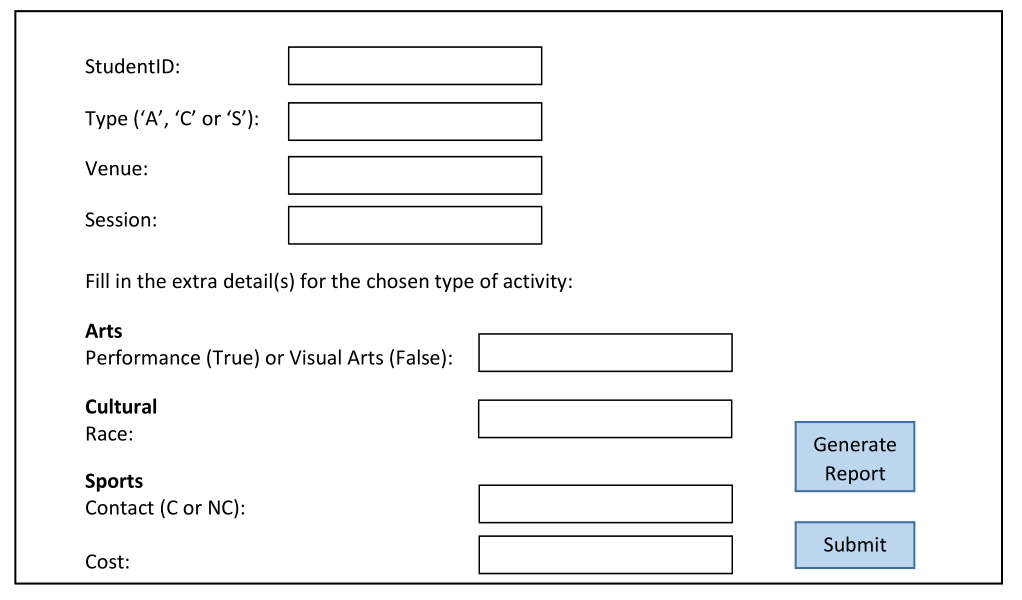
\includegraphics[width=0.5\paperwidth]{C:/Users/Admin/Desktop/Github/question_bank/LyX/static/img/9569-NYJC-2020-P2-Q4}
\par\end{center}

Write a Python program and the necessary files to create a web application
that: 
\begin{itemize}
\item accepts the input from the web form (assume input is keyed in correctly) 
\item updates the registration details into \texttt{register.db} 
\item creates and returns a HTML document that enables the web browser to
display a table tabulating the \texttt{StudentID} and \texttt{Type}
of activity registered for the morning session. 
\end{itemize}
Save your Python program as

\texttt{TASK4\_2\_<your name>.py} with any additional files / sub-folders
as needed in a folder named \texttt{TASK4\_2\_<your name>} \hfill{}{[}12{]}

\subsection*{Task 4.3 }

Test your web application by entering the following records via the
form\textquoteright s submit button: 

\texttt{192701, A, Hall, AM, True }

\texttt{192703, A, MPR, PM, False }

\texttt{192723, S, Field, AM, C, 20 }

\texttt{192803, C, 5-56, AM, Malay }

\texttt{192820, S, 5-60, PM, NC, 15 }

\texttt{193005, C, LT4, PM, Chinese }

\texttt{193006, C, LT4, PM, Chinese} 

Save the output of the program when the user clicks on the \textquotedblleft Generate
Report\textquotedblright{} button as \texttt{TASK4\_3\_<your name>.html}\hfill{}
{[}3{]}

\subsection*{Task 4.4 }

Write SQL code to count the number of different races for the cultural
activities. Run this query. 

Save this code as 

\texttt{TASK4\_4\_<your name>.sql} \hfill{}{[}4{]}